\begin{tikzpicture}

\GraphInit[vstyle=Classic]

\Vertex[empty, x=0, y=0]{p};
\Vertex[Lpos=-90, x=2, y=0, L=$p_{t - 2}$]{ptm2};
\Vertex[Lpos=-90, x=4, y=0, L=$p_{t - 1}$]{ptm1};
\Vertex[Lpos=-90, x=6, y=0, L=$p_{t}$]{pt};
\Vertex[Lpos=-90, x=8, y=0, L=$p_{t + 1}$]{ptp1};
\Vertex[Lpos=-90, x=10, y=0, L=$p_{t + 2}$]{ptp2};
\Vertex[Lpos=-90, x=12, y=0, L=$p_{s - 1}$]{psm1};
\Vertex[Lpos=-90, x=14, y=0, L=$p_{s}$]{ps};

\Edge[style ={-, dashed},labelstyle={above}]({p})({ptm2})
\Edge[style ={-},label={$a_{t - 2}$},labelstyle={above}]({ptm2})({ptm1})
\Edge[style ={-},label={$a_{t - 1}$},labelstyle={above}]({ptm1})({pt})
\Edge[style ={-},label={$a_{t}$},labelstyle={above}]({pt})({ptp1})
\Edge[style ={draw=none},label={$(a_{t + 1})$},labelstyle={below}]({pt})({ptp1})
\Edge[style ={-},label={$a_{t + 1}$},labelstyle={above}]({ptp1})({ptp2})
\Edge[style ={draw=none},label={$(a_{t + 2})$},labelstyle={below}]({ptp1})({ptp2})
\Edge[style ={-, dashed},labelstyle={above}]({ptp2})({psm1})
\Edge[style ={-},label={$a_{s - 1}$},labelstyle={above}]({psm1})({ps})
\Edge[style ={draw=none},label={$(a_{s})$},labelstyle={below}]({psm1})({ps})

\end{tikzpicture}
